\normalsize
\subsection*{Substructuring Method}
\begin{figure}[htbp]
  \begin{center}
    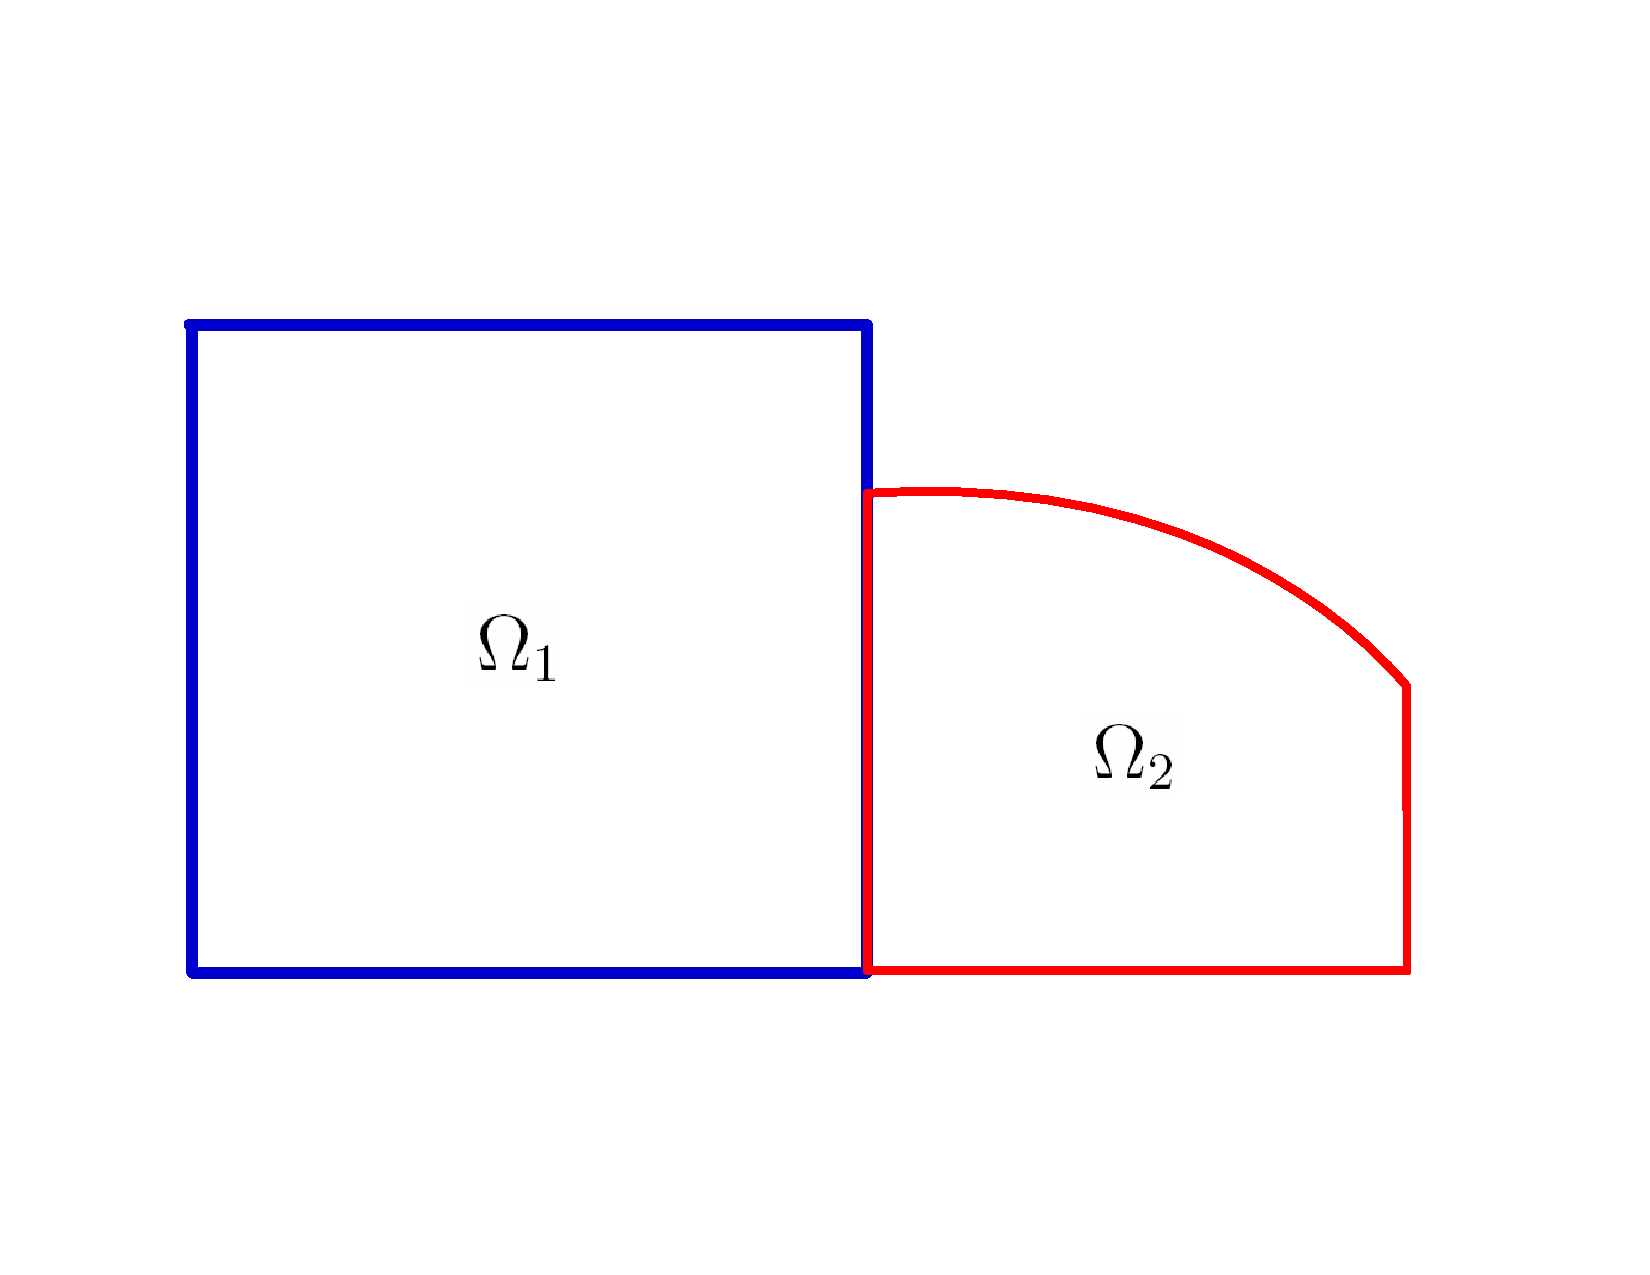
\includegraphics[scale=0.3]{../figures/Nonoverlapping.pdf}
    \caption{Non-Overlapping Method.}
    \label{fig:Nonoverlapping}
  \end{center}
\end{figure}

The linear system obtained from the discretization of the incompressible Navier-Stokes equation can be rearranged such that the unknowns on the interfaces of subdomains can be solved independently from the rest unknowns.

Consider a domain $\Omega$ which is divided into two subdomains $\Omega_1$, $\Omega_2$, and interface $\Gamma$. The system of the discretized partial differential equations for the whole domain $\Omega$ can be written in the matrix form:
\be
\left[
\begin{array}{ccc}
A_{11} & 0 & A_{1\Gamma}\\
0 & A_{22} & A_{2\Gamma}\\
A_{\Gamma 1} & A_{\Gamma 2}  & A_{\Gamma \Gamma}\\
\end{array}
\right]
\left[
\begin{array}{c}
\phi_{1}\\
\phi_{2}\\
\phi_{\Gamma}\\
\end{array}
\right]
=
\left[
\begin{array}{c}
B_{1}\\
B_{2}\\
B_{\Gamma}\\
\end{array}
\right]
\ee
where $\phi_1$ and $\phi_2$ are the variables inside the subdomains, $\phi_{\Gamma}$ contains the variables on the interface $\Gamma$. The system for the variables on the interface can be derived as:
\be
S \ \phi_{\Gamma }=b_{\Gamma}-A_{\Gamma i}A_{i}^{-1}B_i
\label{eqn:Schur-interface}
\ee
where $S$ is the Schur complement of the submatrix $A_{i}$,
\be
S=A_{\Gamma \Gamma}-A_{\Gamma i}A_{i}^{-1}A_{i \Gamma}
\ee
and $A_i$, $A_{\Gamma i}$, $A_{i \Gamma}$, $B_i$ are defined as:
\be
A_i=
\left[
\begin{array}{cc}
A_{11} & 0 \\
0 & A_{22}
\end{array}
\right]
\ee
\be
A_{\Gamma i}=(A_{\Gamma 1},A_{\Gamma 2}), \ \
A_{i \Gamma}=(A_{1 \Gamma},A_{2 \Gamma})^T , \ \
B_i=(B_1,B_2)^T
\ee
After the solution on the interface in Equation \ref{eqn:Schur-interface} is found, the two subdomains can be independently solved with the Dirichlet boundary condition on the interface. Couzy \cite{Couzy1995} demonstrated this technique with the spectral element formulation for incompressible flow simulations.
